% --------------------------------------------------------------------------
% Based on Template for DCASE 2018 technical reports; to be used with:
%          dcase2018_techrep.sty  - DCASE 2018 LaTeX style file, and
%          IEEEbib.bst - IEEE bibliography style file.
% Adapted from spconf.sty and waspaa15.sty
% --------------------------------------------------------------------------

\documentclass{article}
\usepackage{dcase2018_techrep,amsmath,graphicx,url,times,booktabs,tabularx}

% Example definitions.
% --------------------
\def\defeqn{\stackrel{\triangle}{=}}
\newcommand{\symvec}[1]{{\mbox{\boldmath $#1$}}}
\newcommand{\symmat}[1]{{\mbox{\boldmath $#1$}}}


\title{DCASE2018 Bird Audio Detection on a microcontroller}


\name{Jon Nordby}
\address{Norwegian University of Life Sciences\\
Faculty of Science and Technology\\
     jonnord@nmbu.no
}

\begin{document}

\ninept
\maketitle

\begin{sloppy}

\begin{abstract}
TODO
\end{abstract}

\begin{keywords}
Acoustic Event Classification,Random Forests,Wireless Sensor Networks,Continuous Acoustic Monitoring
\end{keywords}


\section{Introduction}
\label{sec:intro}

To support 
For this reason this work focused on.
\cite{dStowell2014}

\cite{dcase2018web}


\section{System description}
\label{sec:system}


\section{Evaluation}
\label{sec:evaluation}

% Below is an example of how to insert images. 
% -------------------------------------------------------------------------
\begin{figure}[t]
  \centering
  \centerline{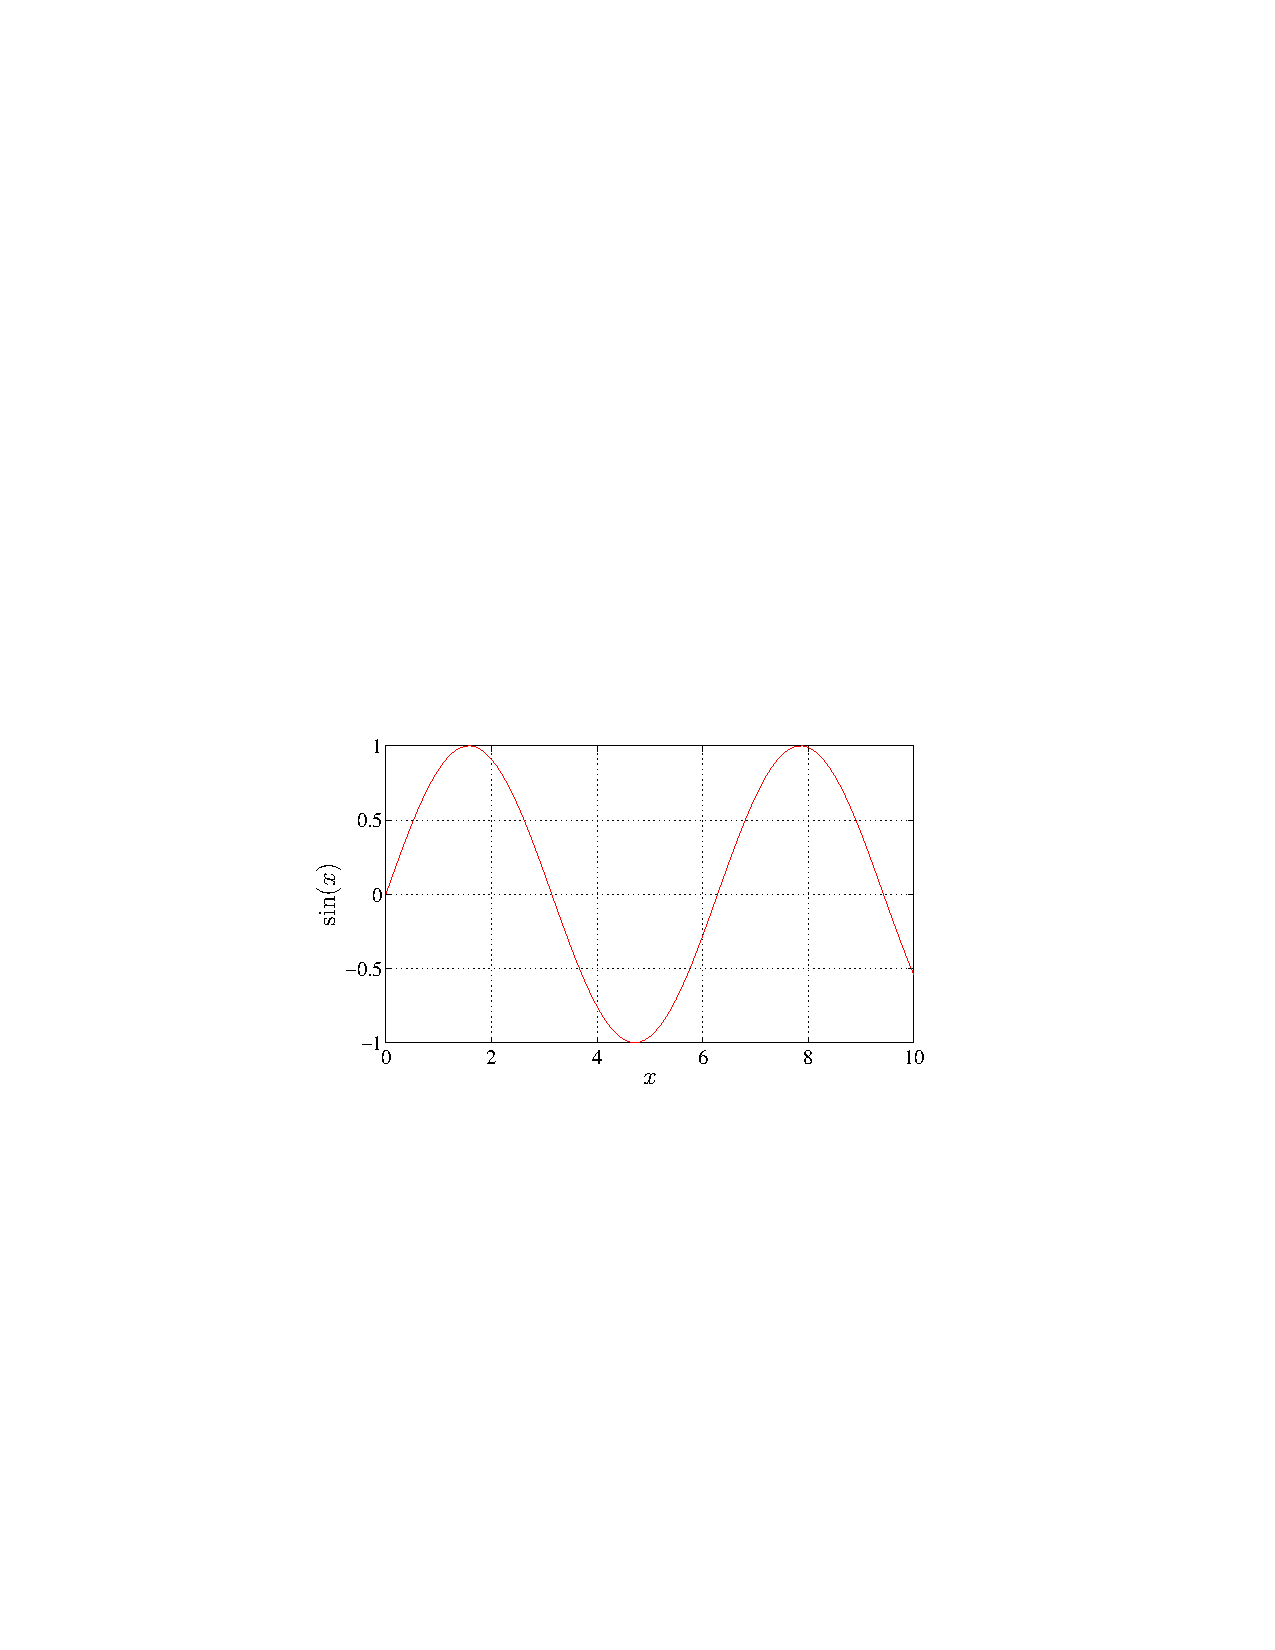
\includegraphics[width=\columnwidth]{fig1a}}
  \caption{Example of a figure with experimental results.}
  \label{fig:results}
\end{figure}


\section{Conclusions}
\label{sec:conclusions}


\subsection{Subheadings}
\label{ssec:subhead}

Fofo


\section{REFERENCES}
\label{sec:ref}



\bibliographystyle{IEEEtran}
\bibliography{refs}

\end{sloppy}
\end{document}
